\section{Analisi armonica e diagrammi di Bode}

\subsection{L'analisi armonica nei sistemi lineari}

Considerando un sistema dinamico $\sum$, asintoticamente stabile, descritto come:
\begin{align}
    \sum_{i=0}^{n} a_i D^i y = \sum_{i=0}^{m} b_i D^i u
\end{align}

($a(s)$ e $b(s)$ sono coprimi fra loro), la funzione di trasferimento è:

\begin{figure}[h!]
    \centering
    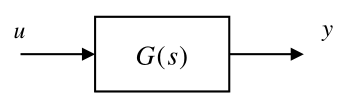
\includegraphics[width=0.3\textwidth]{images/fdt.png}
    \caption{Funzione di trasferimento}
    \label{fig:fdt}
\end{figure}

\begin{align}
    G(s) = \frac{b(s)}{a(s)}
\end{align}



\begin{theorem}
    Sia $\sum$ un sistema asintoticamente stabile con funzione di trasferimento $G(s)$
    razionale.
    La risposta forzata del sistema a un segnale armonico in ingresso è 
    a sua volta un segnale armonico con la stessa frequenza(per $t \to \infty$).
    \`E soddisfatta la relazione:
    \begin{align}
        F(\omega) = G(j\omega)
    \end{align}
\end{theorem}



\subsection{Guadagni del sistema lineare}
Avendo una funzione di trasferimento $G(s)$, si possono individuare i guadagni del sistema:
\begin{itemize}
    \item Guadagno statico: $G(0)$
    \item Guadagno armonico: $|G(j\omega)|$
\end{itemize}


\subsection{Diagrammi di Bode}
Il diagramma di Bode è un grafico che rappresenta il modulo e la fase della funzione di trasferimento
in funzione della pulsazione $\omega$.

Il modulo è rappresentato in scala logaritmica, mentre la fase è rappresentata in scala lineare.
Le varie rappresentazioni sono:
\begin{align}
    G(j\omega) &= | G(j\omega) | e^{j \angle G(j\omega)} \\
    &= | G(j\omega) | \angle G(j\omega)
\end{align}

Nello specifico, il modulo è rappresentato in decibel:
\begin{align}
    db = 20 \log_{10} | G(j\omega) |
\end{align}

Mentre la fase è rappresentata in gradi:
\begin{align}
    \angle G(j\omega) = \arg G(j\omega)
\end{align}


\subsection{Rappresentazioni e parametri della funzione di trasferimento}
Le rappresentazioni della funzione di trasferimento sono \textbf{forma standard con polinomi monici} e  
\textbf{forma standard con poli e zeri}.

La forma standard con polinomi monici è:
\begin{align}
    G(s) = \frac{b(s)}{a(s)} = K_1 \frac{s^m + b_{m-1} s^{m-1} + \dots + b_0}{s_n + a_{n-1} s^{n-1} + \dots + a_0}
\end{align}

Mentre la forma standard con poli e zeri è:
\begin{align}
    G(s) = \frac{b(s)}{a(s)} = K_1 \frac{(s - z_1)(s-z_2) \dots (s-z_m)}{(s-p_1)(s-p_2) \dots (s-p_n)}
\end{align}

In entrambe le forme, $K_1$ è la costante di trasferimento.


\subsection{Parametri caratteristici della risposta armonica}


\begin{table}[h!]
    \centering
    \begin{tabular}{| c | c |}
    \hline
        Pulsazione di risonanza & $\omega_R := \arg \max |G(j\omega)|$ \\
        Picco di risonanza & $M_R := \frac{|G(j\omega_R)|}{|G(j0)|}$ \\
        Larghezza di banda & $ B_{\omega} := \omega_{t2} - \omega_{t1} $ \\
    \hline
    \end{tabular}
\end{table}

$\omega_{t2} > \omega_{t1} \geq 0$ prendono il nome di pulsazioni di taglio e rispettivamente
sono la pulsazione di taglio superiore e quella inferiore.


